\chapter{Theory}
\label{chapter:theory}

In this chapter, all the objects will be considered, for a matter of
simplification, to be smooth i.e. $ C^\infty $. Also, we will use the term
"surface" to refer to any smooth compact hypersurface of $ \R^d $. We will also
call the area of a surface $ \surface $ denoted by $ A(S) $ its $ (d-1)
$-volume. The $ d $-dimensional volume will be denoted by $ Vol^d $. In Chapter
\ref{chapter:2d}, $ Vol^d = Area $ and in Chapter \ref{chapter:3d}, $ Vol^d =
Vol $.

% {{{1 MEAN CURVATURE FLOW
\section{Mean Curvature Flow}

In order to define what we call the Mean Curvature Flow, we will
first need the notions of an embedding and the deformation of a surface:

\begin{definition}
    Let $ S_0 $ be a hypersurface of $ \R^d $. A map $ X: S_0 \to \R^d $ is a
    smooth embedding if it is injective and that $ \forall x\in S_0, $ the
    differential $ D X(x) $ is an injective linear map.
\end{definition}

\begin{definition}
    For a surface $ S_0 \subseteq \R^d $, we call a deformation of $ S_0 $ a
    smooth function $ X : S_0 \times I \to \R^d $ where $ I \subseteq \R $
    (which represents the time) with the following properties:
    \begin{itemize}
        \item $ X(., 0) = id_{S_0} $.
        \item for any $ t \in I $, we denote $ X_t = X(., t) $ and $ S_t =
            X_t(S_0) $. $ X_t $ is an embedding of $ S_0 $ in $ \R^d $.
    \end{itemize}
\end{definition}

Then, the mean curvature flow is a deformation $ X : S_0 \times [0, T] \to \R^d
$ of a surface $ S_0 $ such that:

\begin{equation}
    \partiald{X_t(x)}{t} = \meanv{S_t}(x)
    \label{eqn:mean-curvature-flow}
\end{equation}
where $ \meanv{S_t}(x) $ is the mean curvature vector (see Definition
\ref{prop:curvatures-surface}) of $ S_t $ at $ x $ and $ \partiald{X_t(x)}{t} $
is the normal velocity at $ x $.

In simple words, Equation \ref{eqn:mean-curvature-flow} says that at each step
we move each point of the hypersurface $ S_t $ in the direction of the normal by
an amount given by the mean curvature at this point.

Now, we will recall that the mean curvature flow belongs to a more general
category of geometric flows: the gradient flows (see
\cite{ilmanen1998lectures}). In our case, it follows from the fact that the mean
curvature vector can be identified with the gradient of a certain functional,
namely the area of the surface. The following proposition makes this
identification more rigorous:

\begin{proposition}
    For a surface $ S_0 \subseteq \R^d $ and a deformation $ X : S_0 \times [0, T]
    \to \R^d $ defined by $ X(p, t) = p + t V(p) $ where $ V : \R^d \to \R^d $ is a
    vector field, we have:
    \begin{equation}
        \lim\limits_{t \to 0} \frac{A(S_t) - A(S_0)}{t} = \int_{S_0} V(p)
        \meanv{S_0}(p) dp
    \end{equation}
    where $ A(S) $ denotes the area of the surface $ S $.
    \label{prop:gradient-area-functional}
\end{proposition}

This proposition allows us to identity the gradient of $ A $ to the vector
field associated to the mean curvature vector on $ S_0 $.

To prove this proposition, we will need the next two definitions: the projection
on a hypersurface and the reach of an hypersurface.

\begin{definition}
    For a compact set $ K \subseteq \R^d $, we define the projection of $ x \in
    \R^d $ on $ K $ to be any point $ p \in K $ such that $ || x - p || = d(x,
    K) $.
    The set of all the projections of $ x $ on $ K $ is a subset of $ K $
    that we will denote by $ proj_K(x) $.
\end{definition}

\begin{definition}
    For a compact set $ K \subseteq \R^d $, we define its reach by:
    \begin{equation}
        reach(K) = \max \{ r \geq 0,~\forall x \in R^d \text{ s.t. } d(x, K) \leq
        r,~ card(proj_K(x)) = 1 \}
    \end{equation}
    In other words, the reach is the maximum $ r $ we can take such that the
    projection of any $ x  $ at distance smaller than $ r $ of $ K $ is uniquely
    defined on $ K $.
\end{definition}

The reach has some interesting properties (see \cite{merigot2009detection} for a
more detailed study):

\begin{itemize}
    \item For example, if we consider a circle in the plane of center $ c $ and
        of radius $ R $, then every point in the plane has a unique projection on
        the circle except $ c $ which is at distance $ R $ from every point on the
        circle: $ proj_C(c) = C $. Consequently, its reach is $ R $.

    \item Another more general example is that any convex set has infinite
        reach. This is because the projection on a closed convex set is always
        uniquely defined.

    \item The reach is also related to the Local Feature Size (LFS) introduced
        in \cite{amenta1999surface} for surface reconstruction problems: $
        LFS(p) = d(p, \mathcal{M}) $ $ reach(M) = \min\limits_{p \in M}~LFS(p) $
        where $ \mathcal{M}  $ is the medial axis of $ M $.

    \item The reach is also always upper bounded by the minimum radius of
        curvature. There are no converse result giving a lower bound on the
        reach in term of the curvature. Indeed, consider the
        following example: two spheres of radius $ R $ at distance $ \epsilon $,
        then the radius of curvature is always $ R $ but the reach of the union
        is $ \frac{\epsilon}{2} $.
\end{itemize}

Then, some facts about the curvature of embedded hypersurfaces:

\begin{definition}
    For an hypersurface $ S \subseteq \R^d $, we have:

   \begin{itemize}
       \item the map $ p \in S \rightarrow \vec{n}_S(p) $ where $ \vec{n}_S(p)
           $ is the normal vector of $ S $ at $ p $ is called the Gauss map
           and its differential is called the shape operator. The shape operator
           at $ p $ is a linear map from $ T_p(S) $ to $ T_p(S) $. $ T_p(S) $ is
           the tangent space of $ S $ at $ p $: it is the space which is
           orthogonal to $ \vec{n}_S(p) $. For example, in 3D, $ T_p(S) $ is the
           tangent plane of $ S $ at $ p $.

       \item the shape operator is diagonalizable: its eigenvectors $ P_S^i(p) $
           are called the principal curvature directions and its eigenvalues are
           the $ d-1 $ principal curvatures at $ p $: $ k^1_S(p), \ldots,
           k^{d-1}_S(p) $. So, in the basis formed by $ P_S^i(p) $, the
           matrix of the shape operator is $ diag(k^1_S(p), \ldots,
           k^{d-1}_S(p)) $.

       \item we will also denote $ \meanv{S}(p) $ the mean curvature vector of $
           S $ at $ p $: $ \meanv{S}(p) = \sum_{i=1}^{d-1} k^i_S(p)
           \vec{n}_S(p) $.
   \end{itemize}

   \label{prop:curvatures-surface}
\end{definition}

We will need the notion the $r$-offset of a compact set $ K $:

\begin{definition}
    For $ r > 0 $ and a compact set $ K $, we define the $r$-offset of $ K $
    denoted by $ K^r $ by:
    $$ K^r = \bigcup_{p \in K} B(p, r) $$
\end{definition}

This definition is interesting since the only assumption about $ K $ is that it
is compact, it can either represent a point cloud or a surface.

And finally, we will need the following two lemmas which allow us to compute the
differential of deformations of surfaces.

\begin{lemma}
    \label{lemma:deformation}

    Given a surface $ S $, and a smooth function $ \phi : S \to \R $, we define a
    deformation of $ S $: $ X(p, t) = p + t \phi(p) \vec{n}_S(p) $. Then, we
    have:

    \begin{itemize}
        \item if $ t \leq \frac{reach(S)}{\max \phi} $ then $ X_t $ is an
            embedding of $ S $ in $ \R^d $.
        \item the differential of $ X_t $ at $ p $ is a linear map from $ T_p(S)
            $ to $ \R^d $ and:
            \begin{equation}
                D X_t(p) = p + t D \phi(p) \vec{n}_S(p) + t \phi(p) D \vec{n}_S(p)
            \end{equation}
            In a basis composed of the principal curvature directions of $ S $
            at $ p $ and $ \vec{n}_S(p) $, then we have:
            \begin{equation}
                D X_t(p) =
                \begin{pmatrix}
                    1 + t \phi(p) k^1_S(p) & \cdots & 0 \\
                    \vdots                 & \ddots & \vdots                      \\
                    0                      &        & 1 + t \phi(p) k^{d-1}_S(p)  \\
                    \multicolumn{3}{c}{1 + t D\phi(p)} \\
                \end{pmatrix}
            \end{equation}
        \item For any function $ \chi : X_t(S) \to \R $, we have the following
            change of variable result:
            \begin{equation}
                \int_{X_t(S)} \chi(x) dx = \int_S \chi(X_t(p)) J_{X_t}(p) dp
            \end{equation}
            where $ J_{X_t}(p) = (1 + t \phi(p) k^1_S(p)) \hdots (1 + t \phi(p)
            k^{d-1}_S(p)) $ is the Jacobian of $ X_t $ at $ p \in S $.
    \end{itemize}
\end{lemma}

\begin{lemma}
    \label{lemma:diffeo}

    Given a surface $ S $, $ r = reach(S) $, and a deformation $ f : S \times
    [-r, r] \to \R^d $ defined by $ F(p, t) = p + t \vec{n}_S(x) $, then:

    \begin{itemize}
        \item $ F $ is a diffeomorphism from $ S \times [-r, r] $ to $ S^r $
        \item the differential of $ F $ at $ p $ is a linear map from $ T_p(S)
            \times \R $ to $ \R^d $. In the basis formed by the principal
            curvature directions at $ p $ and the normal $ \vec{n}_S(p) $, we have:
            \begin{equation}
                D F(p, t) = diag(1 + t k^1_S(p), \ldots, 1 + t k^{d-1}_S(p), 1)
            \end{equation}
            So its Jacobian is:
            \begin{equation}
                J_F(p, t) = \prod_{i=1}^{d-1} (1 + t k^i_S(p))
            \end{equation}
        \item For any function $ \chi : S^r \to \R $, we have the following
            change of variable result:
            \begin{equation}
                \int_{S^r} \chi(x) dx = \int_S \int_{-r}^r \chi(F(p, t)) J_F(p,
                t) dt dp
            \end{equation}
    \end{itemize}
\end{lemma}

Then, we can tackle the proof of the proposition
\ref{prop:gradient-area-functional}.

\begin{proof}[Sketch of proof of Proposition \ref{prop:gradient-area-functional}]
    We use the deformation $ X : S_0 \times [0, T] $ where $ X(p, t) = p + t
    \phi(p) \vec{n}_{S_0}(p) $ for $ \phi : S_0 \to \R $ is a smooth
    function. Then, we have, using the lemma \ref{lemma:deformation} with $ \chi
    = 1 $:

    \begin{align*}
        A(S_t) &= \int_{S_t} 1 dx = \int_{S_0} J_X(p) dp \\
        &= \int_{S_0} \prod_{i=1}^{d-1} (1 + t \phi(p) k^i_{S_0}(p)) \\
        &= \int_{S_0} 1 dp + t \int_{S_0} \phi(p) \meanv{S_0}(p) dx + O(t^2) \\
        &= A(S_0) + t \int_{S_0} \phi(p) \meanv{S_0}(p) dx + O(t^2)
    \end{align*}

    So:
    $$ \lim\limits_{t \to 0} \frac{A(S_t) - A(S_0)}{t}= \int_{S_0}
    \phi(p) \meanv{S_0}(p) dp $$

    This equation tells us exactly that if we perturb a surface by $ \phi $
    then the variation of the area functional is linked to the mean curvature.
    In other words, $ \meanv{S_0} $ is the $ L^2 $ gradient of the area
    functional.
\end{proof}

This proposition will be at the basis of our work. We will discretize the
hypersurface by taking points sampled on it and try to approximate the area of
the hypersurface by something which can be computed using only the point cloud.

% {{{1 DISCRETIZATION OF THE AREA
\section{Discretization of the area}

In this section, we will try to compute an approximation of the area of an
hypersurface with knowing only points sampled on it. We can relate the area of
an hypersurface to the volume of its tubular neighbourhood using a variant of
the tube formula \cite{weyl1939volume}.

\begin{proposition}
    \label{prop:comp-offset-area}
    If $ S $ is a smooth hypersurface whose reach is positive and $ reach(S) > r
    > 0 $, then:
    \begin{equation}
        A(S) = \frac{Vol^d(S^r)}{2r} + O(r^2)
    \end{equation}

    The constants in the error term of the development only depend on the curvature
    of $ S $.
\end{proposition}

\begin{proof}
    We have: $ Vol^d(S^r) = \int_{S^r} 1 dx $. Now, we will use the
    following deformation: $ X(p, t) = p + t \vec{n}_{S}(p) $ Using this
    substitution and Lemma \ref{lemma:diffeo} with $ \chi = 1 $:

    \begin{align*}
        Vol^d(S^r) &= \int_S \int_{-r}^r J_f(p) dt dp \\
        &= \int_S \int_{-r}^r \prod_{i=1}^{d-1} (1 + t \kappa_i(p)) dt dp \\
        &= \int_S \int_{-r}^r \left( 1 + \sum_{k=1}^{d-1} t^k \sum_{i_1 < \ldots
                < i_k} \kappa_{i_1}(p) \ldots \kappa_{i_k}(p) \right) dt dp \\
        &= 2r \int_S 1 dp + \int_K \int_{-r}^r \sum_{k=1}^{d-1} t^k \sum_{i_1 < \ldots < i_k} \kappa_{i_1}(p) \ldots \kappa_{i_k}(p) dt dp \\
        &= 2r A(S) + O(r^2)
    \end{align*}

    So: $ \frac{Vol^d(S^r)}{2r} = A(S) + O(r^2) $.
\end{proof}

This proposition is related to the Minkowski content. It is used to measure the
area of the boundary of a set: the $ d-1 $ dimensional volume in dimension $ d
$. It is defined as follows:
$$ \lim\limits_{\epsilon \to 0} \frac{Vol^d(S^{\epsilon}) - Vol^d(S)}{\epsilon} $$

This is exactly what we computed: a Taylor expansion of $ Vol^d(S^r) $.

Next, we want to approximate $ Vol^d(S^r) $ by $ Vol^d(P^r) $ where $ P \subset
S $ is a point cloud. We will need a formalization of the notion of sampling:

\begin{definition}
    A set of points $ p_i $ is said to be an $\epsilon$-sampling of a manifold $
    M $ if the set of the balls  $ B(p_i, \epsilon) $ verifies: $ M \subseteq
    \bigcup_i B(p_i, \epsilon) $ (see \cite{amenta1999surface}).
\end{definition}

The following proposition bounds the error of this approximation:

\begin{proposition}
    \label{prop:comp-vol-offsets}
    For an hypersurface $ S $ with positive reach and an $\epsilon$-sampling $ P
    \subseteq S $, we have:
    \begin{equation}
        0 \leq Vol^d(S^r) - Vol^d(P^r) \leq \frac{\epsilon^2}{r} A(S) +
        O(\frac{\epsilon^4}{r^2})
    \end{equation}
\end{proposition}

\begin{proof}
    Since $ P \subseteq S $, then $ Vol^d(S^r) \leq Vol^d(P^r) $. Then, we
    parametrize the boundary of $ P^r $ by $ f : S \to \partial P^r $ where $
    f(p) = p + r(p) \vec{n}_S(p) $ for $ r(p) \in [0, r] $ (see Figure
    \ref{fig:offset-parametrization}).

    \begin{figure}[h]
        \centering
        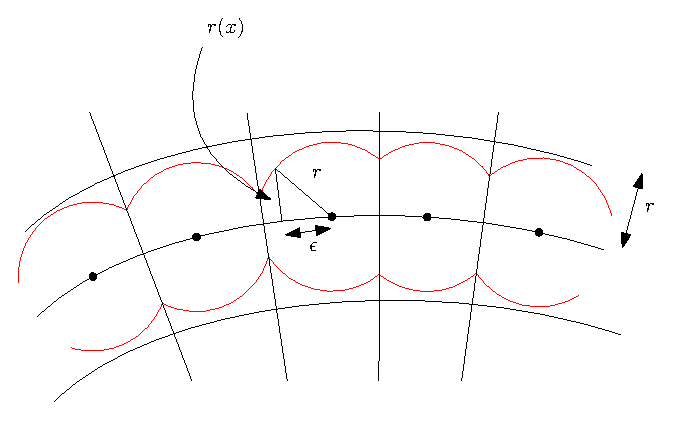
\includegraphics[scale=0.8]{offset-parametrization}
        \caption{Parametrization of the offset (in red)}
        \label{fig:offset-parametrization}
    \end{figure}

    We have:
    \begin{align*}
        r(p)^2 + \epsilon^2 = r^2 \iff& (r - r(p)) (r + r(p)) = \epsilon^2 \\
        \iff& r - r(p) = \frac{\epsilon^2}{r + r(p)} \leq \frac{\epsilon^2}{r} \\
    \end{align*}

    Now, we will use the same formula as in the previous proofs:

    \begin{align*}
        Vol^d(S^r) - Vol^d(P^r) &= \int_{S^r \textbackslash P^r} 1 dp \\
        &= \int_S \int_{r(p)}^r J_f(p, t) dt dp \\
        &= \int_S \int_{r(p)}^r \left( 1 + \sum_{k=1}^{d-1} t^k \sum_{i_1 < \ldots
                < i_k} k^{i_1}_S(p) \ldots S^{i_k}_S(p) \right) dt dp \\
        &= \int_S (r - r(p)) dp + O((r - r(p))^2) \\
        &\leq \frac{\epsilon^2}{r} A(S) + O(\frac{\epsilon^4}{r^2}) \qedhere
    \end{align*}
\end{proof}

Now, combining the previous propositions, we will show that we can approximate
the area of $ S $ by the volume of $ P^r $:

\begin{proposition}
    \label{prop:approx-volume-area}
    Given an hypersurface $ S $, an $\epsilon$-sampling of $ S $: $ P $, we
    have:
    \begin{equation}
        | \frac{Vol^d(P^r)}{2r} - A(S) | \leq \frac{\epsilon^2}{2r^2} +
        O(\frac{\epsilon^4}{r^3}) + O(r^2)
    \end{equation}

    So, when $ \frac{\epsilon}{r} $ and $ r $ vanish then $
    \frac{Vol^d(P^r)}{2r} $ converges towards the area of $ S $.
\end{proposition}

\begin{proof}
    We will use the propositions \ref{prop:comp-vol-offsets} and
    \ref{prop:comp-offset-area}. We have, using the triangle inequality:
    \begin{align*}
        \left| \frac{Vol^d(P^r)}{2r} - A(S) \right| \leq& \left| \frac{Vol^d(P^r)}{2r} -
            \frac{Vol^d(S^r)}{2r} \right| + \left| \frac{Vol^d(S^r)}{2r} -
            A(S) \right| \\
        \leq& \frac{\epsilon^2}{2r^2} A(S) + O(\frac{\epsilon^4}{r^3}) + O(r^2)
        \qedhere
    \end{align*}
\end{proof}

At this point, we have shown a way to approximate the area of an hypersurface
with a quantity proportional to the volume of the $r$-offset of a point cloud
sampled on the surface.
Now, we want to study the gradient of this newly computed quantity.

% {{{1 CONVERGENCE OF THE GRADIENT
\section{Convergence of the gradient}

In this section, we will consider the functional $ A^r : \R^d, \hdots, \R^d \to
\R $ defined as follows:

\begin{equation}
    A^r(p_1, \ldots, p_N) = Vol^d(\bigcup_{i=1}^N B(p_i, r)
\end{equation}

We will derive formulae for the gradients of $ A^r $. First, we will define what
we mean by "gradients":

\begin{definition}
    If $ F : (\R^d)^N \to \R $ is a function over $d$-dimensional point clouds,
    and $ p \in (\R^d)^N $, then the $j$-th ($ j \in \{1, \ldots, d\} $)
    coordinate of $ \nabla_{p_i} F(p) \in \R^d $ for $ i \in \{1, \ldots, N\} $
    is given by:

    $$ (\nabla_{p_i} F(p))_j = \lim\limits_{\epsilon\to 0} \frac{F(p_1,\ldots,p_i+
    \epsilon e_j, \ldots, p_N) - F(p)}{\epsilon} $$
    where $ (e_1, \ldots, e_d) $ is the standard basis of $ \R^d $.
\end{definition}

The next proposition gives the gradient of the volume of union of balls :
\begin{proposition}
    The gradient of the functional $ A^r $ at a point $ p = (p_1, \ldots, p_N) $
    is given by:

    \begin{equation}
        \label{eqn:gradient_area_2d}
        \nabla_{p_i} A^r(p) = \int_{B} \frac{x - p_i}{||x - p_i||} dx
    \end{equation}
    where $ B = \partial B(p_i, r) \cap V(p_i, P) $ is the visible boundary of
    the ball.
\end{proposition}

Note that \cite{lachand2005minimizing} tackles the problem of minimizing a
functional over the set of convex bodies. For doing this, the authors compute the
derivatives of this functional: we use a similar technique to prove our
proposition.

\begin{proof}

For this proof, we will use Formula \ref{eqn:area-union-balls}. Assume that we
move the point $ p_i $ by a small quantity $ \delta p_i $, let us study the
variation of the area of $ \bigcup_i V(p_i, P) \cap B(p_i, r) $.

More formally, let us define $ A_{\epsilon} = A(V(p_i + \epsilon \delta p_i, P) \cap
B(p_i + \epsilon \delta p_i, r)) $, we want to compute the following limit:
$$ \lim\limits_{\epsilon \to 0} \frac{A_{\epsilon} - A_0}{\epsilon} $$

To compute this quantity, we will define the following sets:
\begin{itemize}
    \item $ B_1 = \{ x \in B, (x - p_i | \delta p_i) \geq 0\} $
    \item $ \mathcal{A}^1_{\epsilon} = \bigcup_{x \in B_1} [x, x + \epsilon \delta p_i] $:
        "upper" gained area (see Figure \ref{fig:demo-gradient} for a drawing of the
        situation in 2D)
    \item $ B_2 = \{ x \in B, (x - p_i | \delta p_i) \leq 0\} $
    \item $ \mathcal{A}^2_{\epsilon} = \bigcup_{x \in B_2} [x, x + \epsilon \delta p_i] $:
        "lower" lost area.
\end{itemize}

\begin{figure}[h]
    \centering
    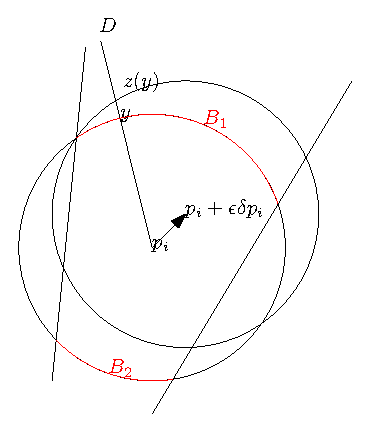
\includegraphics[scale=0.8]{2d/2d_proof_gradient_area}
    \caption{Situation for a ball $ B(p_i, r) $ in 2D}
    \label{fig:demo-gradient}
\end{figure}

Then, we have: $ A_\epsilon = A_0 + Vol(\mathcal{A}^1_\epsilon) -
Vol(\mathcal{A}^2_\epsilon) + O(\epsilon^2) $

Now, we will evaluate $ Vol(\mathcal{A}^1_\epsilon) $, we will do similarly for $
Vol(\mathcal{A}^2_\epsilon) $.

For any $ x \in B $, we define $ z(x) $ as the intersection of the half-line $ D
$ (see Figure \ref{fig:demo-gradient}) with the circle of center $ p_i +
\epsilon \delta p_i $ of radius $ r $. We also parametrize the half-line $ D $
by: $ x + t \frac{x - p_i}{||x - p_i||} $ for $ t \ge 0 $.

Let us find this intersection point $ z(x) $, we assume that $ t $ is small by
neglecting second order terms $ O(t^2) $. We need to find $ D \cap C(p_i +
\delta p_i, r) $. Let $ t \ge 0 $ then, we have :

\begin{equation}
    || x + t \frac{x - p_i}{||x - p_i||} - (p_i + \epsilon \delta p_i) ||^2 = r^2
    \tag{$\star$}
\end{equation}

If we expand this expression, we get:

\begin{align*}
    (\star) & \iff || x - (p_i + \epsilon \delta p_i) ||^2 + t^2 + 2t \left(
        \frac{x-p_i}{|| x - p_i||} | x - (p_i + \epsilon \delta p_i) \right) = r^2 \\
    & \iff || x - p_i || ^2 - 2 \epsilon (x - p_i | \delta p_i) + || \epsilon \delta p_i || ^2 + t^2 + 2t
    \left( \frac{x-p_i}{|| x - p_i||} | x - (p_i + \epsilon \delta p_i) \right) = r^2 \\
    & \iff -2 \epsilon (x - p_i | \delta p_i) + 2t || x - p_i|| + o(\epsilon^2) = 0
    \text{ because } || x - p_i || = r \\
    & \iff t = t^{\star} = \epsilon \left( \frac{x - p_i}{||x - p_i||} | \delta p_i \right) +
    o(\epsilon^2)
\end{align*}

Then, $ z(y) = x + t^{\star} \frac{x - p_i}{||x - p_i||} $ and $ || x - z(x) || =
t^{\star} $.

We deduce that :
$$ Vol(\mathcal{A}^1_\epsilon) = \int_{B_1} || x - z(x) || dx = \int_{B_1}
\left[ \epsilon \left( \frac{x - p_i}{||x - p_i||} | \delta p_i \right) +
    o(\epsilon^2) \right] dx $$

And:

$$ Vol(\mathcal{A}^1_\epsilon) - Vol(\mathcal{A}^2_\epsilon) = \int_{B} \left[
    \epsilon \left( \frac{x - p_i}{||x - p_i||} | \delta p_i \right) +
    o(\epsilon^2) \right] dx $$

Finally, we have, by linearity:
\begin{equation*}
    \nabla_{p_i} A^r(p) = \int_{B} \frac{x - p_i}{||x - p_i||} dx \qedhere
\end{equation*}

\end{proof}

Now, we will relate the previously computed gradients to the mean curvature
vector of an hypersurface. If we suppose that we have a point cloud that is an
$\epsilon$-sampling of a smooth hypersurface $ S $, then the following
proposition gives the link between the gradient of volume of an offset of $ S $
and the mean curvature vector.

\begin{proposition}
    Given an $\epsilon$-sampling $ P $ of a smooth ($ C^{\infty} $) hypersurface
    $ S $ and $ r \ge 0 $ such that: $ \epsilon \leq r \leq reach(M) $, then,
    for $ p = (p_1, \ldots, p_N) \in P^N $:
    \begin{equation}
        \frac{\nabla_{p_i} A^r(p)}{r \times Vol^{d-1}(\partial B(p_i,r) \cap V(p_i,P))}
        = \meanv{S}(p_i) + O \left(\frac{\epsilon}{r}\right) + O(r)
    \end{equation}
    Consequently, when $ r $ and $ \frac{\epsilon}{r} $ vanish then $
    \nabla_{p_i} A^r(p) $ converges towards a quantity proportional to the
    mean curvature vector of $ S $ at $ p_i $.
    \label{prop:gradient-mean-curvature}
\end{proposition}

To prove that, we will need two lemmas extracted from \cite{amenta1999surface}
which will tell us how the Voronoi cells look:
\begin{lemma}
    If $ S $ is an hypersurface, $ P $ an $\epsilon$-sampling of $ S $ and $ p
    \in P $, then:
    $$ V(p, P) \cap S \subseteq B\left(p, \frac{\epsilon}{1 - \epsilon}
        LFS(p)\right) $$
\end{lemma}

\begin{lemma}
    If $ S $ is an hypersurface, $ P $ an $\epsilon$-sampling of $ S $, $ p \in
    P $ and $ v \in V(p, P) $ such that $ d(p, v) \ge \alpha LFS(p) $ for $
    \alpha > 0 $, then the angle at $ s $ between the vector $ v $ and the
    normal at the surface (oriented in the same direction) is at most $
    \arcsin(\frac{\epsilon}{\alpha(1-\epsilon)}) +
    \arcsin(\frac{\epsilon}{(1-\epsilon)}) $.
\end{lemma}

These two lemmas tell us that the Voronoi cells are skinny (first lemma) and
long (second lemma).

\begin{proof}[Proof of Proposition \ref{prop:gradient-mean-curvature}]
We will first do two approximations on the equation \eqref{eqn:gradient_area_2d}:
\begin{enumerate}
    \item the first one is to suppose that the offset of $ S $ is close enough
        to the offset of $ P $. Using the computation done in
        \ref{prop:comp-vol-offsets}, we can say that the error made is in the
        order of $ O(\frac{\epsilon^2}{r}) $.
    \item the second one is that if the sampling is dense enough then we can
        replace $ p_i $ by the projection of $ x \in V(p_i, P) $ on $ S $: $
        \forall x \in V(p_i, P),~p_i = p_S(x) + O(\epsilon) $, see Figure
        \ref{fig:voronoi-cylinder}.  For this approximation to hold, it is
        necessary for the pointed out distance to be greater than $ \epsilon $
        i.e. $ r \gg \epsilon $ which means that $ \frac{\epsilon}{r} $ needs to
        vanish. This will allow us to say that: $ || x - p_i || = O(r) $.
\end{enumerate}

\begin{figure}[h]
    \centering
    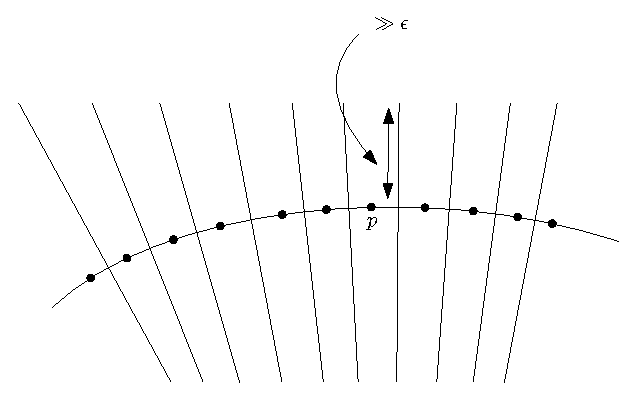
\includegraphics[scale=0.6]{img/voronoi-cylinder}
    \caption{Shape of the Voronoi cells of densely sampled points}
    \label{fig:voronoi-cylinder}
\end{figure}

Using these approximations, we get:
\begin{align*}
    \int_{\partial{P^r} \cap V(p_i, P)} (x - p_i) dx & \stackrel{(1)}{=}
    \int_{\partial{S^r} \cap V(p_i,
        P)} (x - p_i) dx + O(\epsilon^2) \\
    &\stackrel{(2)}{=} \int_{\partial{S^r} \cap V(p_i, P)} (x - p_S(x)) dx +
    O(\epsilon) \\
\end{align*}

Then, we will use the substitution $ q = p_S(x) \iff x = F^{+}(q) = q +
r \vec{n}_S(q) $ on the upper part of $ \partial{S^r} \cap V(p_i, P) $. Using
the lemma \ref{lemma:diffeo}, we have that $ F^{+} $ is a diffeomorphism and that
$ J_{F^+}(q) = (1 + r k^1_S(q)) \hdots (1 + r k^{d-1}_S(q)) $.

Using an analogous substitution on the lower part of $ \partial{S^r} \cap V(p_i,
P) $, we get : $ J_{F^-}(q) = (1 - r k^1_S(q)) \hdots (1 - r k^{d-1}_S(q)) $. By
subtracting the two, we obtain: $ 2 r \mean{S}(q) + O(r^2) $.

It follows that:
\begin{align*}
    \int_{\partial{S^r} \cap V(p_i, P)} (x - p_S(x)) dx &= \int_{S \cap V(p_i, P)}
    \vec{n_S}(q) ( J_{F^+}(q) -J_{F^-}(q) ) dq \\
    &= 2r \int_{S \cap V(p_i, P)} \meanv{S}(q) dq + O(r^2) \\
\end{align*}

Finally, since we have supposed that $ S $ is $ C^{\infty} $ then, we can write:
$ \vec{n_S}(q) = \vec{n_S}(p_i) + O(\epsilon) $, $ \meanv{S}(q) = \meanv{S}(p_i)
+ O(\epsilon) $. Error terms are negligible since they depend on the third derivative
of the curvature. We deduce that:

$$ \nabla_{p_i} A^r(p) = 2r \meanv{S}(p_i) \int_{S \cap V(p_i, P)} 1 dq + O(r^2)
+ O(\epsilon) $$

Then, we can write:

$$ \int_{S \cap V(p_i, P)} 1 dq = Vol^{d-1}(S\cap V(p_i,P)) \simeq \frac{1}{2}
    Vol^{d-1}(\partial B(p_i,r) \cap V(p_i,P)) $$

So:
\begin{equation*}
    \frac{\nabla_{p_i} A^r(p)}{r \times Vol^{d-1}(\partial B(p_i,r) \cap V(p_i,P))}
    = \meanv{S}(p_i) + O \left(\frac{\epsilon}{r}\right) + O(r) \qedhere
\end{equation*}

\end{proof}

We can summarize the situation with the following diagram:

\begin{displaymath}
    \xymatrix{A^r \ar[d]^{\nabla} \ar[r] & A \ar[d]^{\nabla} \\
        \nabla A^r \ar[r] & \nabla A }
\end{displaymath}

$ A^r $ represents the discretization of the area of an hypersurface: it
is $ \frac{Vol^d(P^r)}{2r} $ which converges towards the continuous area (see
Proposition \ref{prop:approx-volume-area}). There is also a convergence property
for the gradients: the discretized gradient converges towards the continuous one
(see Proposition \ref{prop:gradient-mean-curvature}).

In some sense, "discretization" and "gradient" commute: the gradient of the
discretization converges towards the continuous gradient.

% {{{1 OTHER KINDS OF DISCRETIZATIONS
\section{Other kinds of discretizations}

% TODO: flot de l'aire du bord d'une surface = union de boules

In this work, we were also interested in other discretizations. Instead of
choosing the volume as the functional, we can also choose the area of the
boundary or corresponding weighted versions (i.e. the gradient of the volume
will be weighted by the corresponding volume of the intersection between the
Voronoi cell and a ball).

For the former case (area of the boundary), we have the following lemma:
\begin{lemma}
    If $ S $ is a smooth hypersurface whose reach is positive and $ reach(S) > r
    > 0 $, then:
    \begin{equation}
        A(S) = \frac{Vol^d(\partial S^r)}{2r} + O(r^2)
    \end{equation}
\end{lemma}

During this internship, we did not prove that the gradients of the area of the
boundary of a union of balls are directly connected (like for the volume of the
union) to the mean curvature of the sampled surface. But even if we did not
made the prove, we made experiments to show this relation.

Finally, we were interested in replacing the Euclidean ball with a convex
polyhedron in order to have an anisotropic smoothing. A more detailed study of
this problem will be done in the next section.

% {{{1 3D CASE
\section{3D case}
\label{sec:theory-3d-case}

In this section, we will study the influence of the choice we made by replacing,
in chapter \ref{chapter:3d}, the Voronoi diagram computed with a polyhedral norm
with the standard one. We will show that the function that we minimized is not
the volume of the union of convex polyhedra but another functional. For this, we
will need the definition of the radial function of a convex set:

\begin{definition}
    For a convex set $ K $, we define the radial function $ \rho_K $ by:
    $$ \rho_K(x) = \sup \{ r \in \R,~rx \in K \} $$
\end{definition}

For a surface $ S $ and a deformation $ X(p, t) = p + t \vec{n}_S(p) $ for $ t \in
[-r \rho_K(-\vec{n}_S(p)), r \rho_K(\vec{n_S}(p)) ] $, let us denote by $ A' $
the following functional:

\begin{equation}
    A'(S) = \int_S \int_{-r \rho_K(-\vec{n}_S(p))}^{r \rho_K(\vec{n_S}(p))}
    J_X(p, t) dt dp
\end{equation}
where $ K $ is a convex polyhedron.

We have, in 3D, using the lemma \ref{lemma:diffeo}:

\begin{align*}
    A'(S) &= \int_S \int_{-r \rho_K(-\vec{n}_S(x))}^{r \rho_K(\vec{n_S}(x))}
    \left[ 1 + (\kappa_1(x) + \kappa_2(x)) t + \kappa_1(x) \kappa_2(x) t^2
    \right] dt dx \\
    &= \int_S (r \rho_K(\vec{n_S}(x)) + r \rho_K(-\vec{n_S}(x))) dx + O(r^2)
\end{align*}

Now, if $ K $ is symmetric, i.e. if $ x \in K $ then $ -x \in K $ which implies
that $ \rho_K(\vec{n_S}(x)) = -\rho_K(-\vec{n_S}(x)) $, then we get:

\begin{equation}
    A'(S) = 2r \int_S \rho_K(\vec{n}_S(x)) dx + O(r^3)
\end{equation}

So:
\begin{equation}
    \frac{1}{2r} A'(S) = \int_S \rho_K(\vec{n}_S(x)) dx + O(r^2)
\end{equation}

Thus, the functional we minimized is $ A' $ and not the volume of the union.

% vim: set spelllang=en :
